Feed-forward network (FFN), the first invented ANN and the simplest variation of an ANN. Its name comes from the way how information flows through the network. The data flows in one direction, oriented from the \textit{input layer} to the \textit{output layer}, without cycles. The input layer takes input data, vector $\vec{x}$, producing $\hat{y}$ at the output layer \cite{ffnbrilliant}.

FFN contains several hidden layers of various widths but it can also have no hidden layers at all. By having no back-loops, FFN generally minimizes error, computed by \textit{cost function}, in its prediction by using the \textit{backpropagation} algorithm to update its weight values \cite{mainTypesANN}, \cite{lipton2015critical}.

\begin{figure}[h]
    \centering
    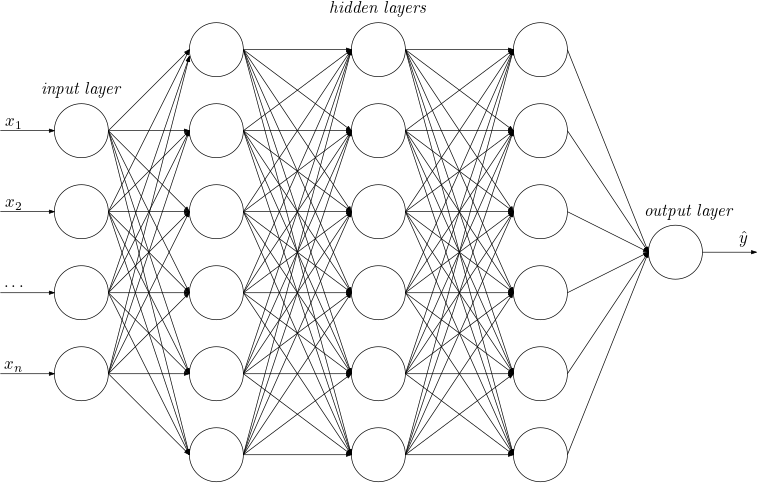
\includegraphics[width=12cm]{ffn.png}
    \caption{Fully connected Feed-forward Neural Network \cite{matous}}
    \label{fig:ffn}
\end{figure}

%=======================================================================================================================

\subsubsection{Cost Function}
Cost function $C(\vec{w})$ is used in ANN's training process. It takes all weights and biases of an ANN as its input, in the form of a vector $\vec{w}$ and calculates a single real number expressing ANN's error in prediction \cite{Goodfellow-et-al-2016}. Higher number expressing poor prediction and as the number gets lower the ANN's output gets closer to the correct result. The main goal of training is to minimize the cost function. 

%=======================================================================================================================
\subsubsection{Backpropagation}
Backpropagation, short of backward propagation of errors, is a widely used algorithm in training FFN using \textit{gradient descent} to find a local minimum of a cost function and update ANN's weights \cite{birlliantbackprop}.

The gradient of a multi-variable function provides us with the direction of the gradient ascent, where we should step to rapidly increase the output and find the local maximum. Conversely, the negative of the gradient points towards the local minimum.'

It is common practice to split training samples into small \textit{batches} of size $n$. For each sample in the batch, we will calculate a gradient descent and use their average gradient descent to update the network's weights. This average gradient descent indicates the adjustments that need to be made to the weights so that the artificial neural network (ANN) moves closer to the correct results \cite{birlliantbackprop}.

\begin{equation}
    {- \gamma \nabla C(\vec{w}_i) + \vec{w}_i \rightarrow \vec{w}_{i+1} }
\end{equation}

$\vec{w_i}$ is weights of the network at the current state (batch), $\vec{w_{i+1}}$ is updated weights, $\gamma$ is the learning rate and $-\nabla C(\vec{w_i})$ is the gradient descent.
